\begin{figure}[!htb]
\centering
  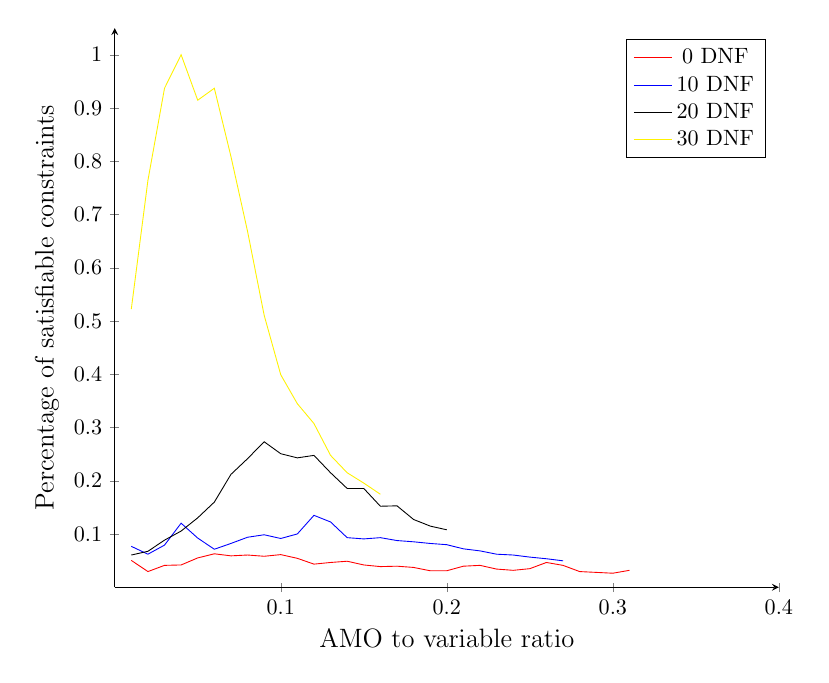
\begin{tikzpicture}[>=latex, scale=0.8]
\centering
\begin{axis}[
  cycle list name=color list,
  axis x line=center,
  axis y line=center,
  width={\linewidth},
  xtick={0,0.1,...,0.35},
  ytick={0.1,0.2,...,1},
  xlabel={AMO to variable ratio},
  ylabel={Percentage of satisfiable constraints},
  every axis x label/.style=
            {at={(ticklabel cs: 0.5,0)}, anchor=north},
  every axis y label/.style=
            {at={(ticklabel cs: 0.5,0)}, anchor=south},
  ylabel style={rotate=90},
  label style={font=\large},
  xmin= 0,
  xmax=0.4,
  ymin=0,
  ymax=1.05]

  \addplot+ [no marks] table {
0.01 0.05046583850931677
0.02 0.029503105590062112
0.03 0.04114906832298137
0.04 0.04192546583850932
0.05 0.05512422360248447
0.06 0.06288819875776397
0.07 0.059006211180124224
0.08 0.06055900621118013
0.09 0.05822981366459627
0.1 0.06133540372670807
0.11 0.05434782608695652
0.12 0.043478260869565216
0.13 0.046583850931677016
0.14 0.04891304347826087
0.15 0.04192546583850932
0.16 0.03881987577639751
0.17 0.039596273291925464
0.18 0.037267080745341616
0.19 0.031055900621118012
0.2 0.031055900621118012
0.21 0.039596273291925464
0.22 0.04114906832298137
0.23 0.034161490683229816
0.24 0.03183229813664596
0.25 0.03493788819875776
0.26 0.046583850931677016
0.27 0.04114906832298137
0.28 0.029503105590062112
0.29 0.027950310559006212
0.3 0.026397515527950312
0.31 0.03183229813664596
};

  \addplot+ [no marks] table {
0.01 0.07686335403726709
0.02 0.062111801242236024
0.03 0.07919254658385093
0.04 0.1203416149068323
0.05 0.09239130434782608
0.06 0.07142857142857142
0.07 0.08229813664596274
0.08 0.09394409937888198
0.09 0.0986024844720497
0.1 0.09161490683229814
0.11 0.10015527950310558
0.12 0.13509316770186336
0.13 0.12267080745341614
0.14 0.09316770186335403
0.15 0.09083850931677019
0.16 0.09316770186335403
0.17 0.08773291925465838
0.18 0.08540372670807453
0.19 0.08229813664596274
0.2 0.07996894409937888
0.21 0.07220496894409938
0.22 0.06832298136645963
0.23 0.062111801242236024
0.24 0.06055900621118013
0.25 0.056677018633540376
0.26 0.05357142857142857
0.27 0.049689440993788817

};

\addplot+ [no marks] table {
0.01 0.06055900621118013
0.02 0.06754658385093168
0.03 0.08850931677018634
0.04 0.10559006211180125
0.05 0.13043478260869565
0.06 0.15993788819875776
0.07 0.21195652173913043
0.08 0.24145962732919254
0.09 0.2732919254658385
0.1 0.25077639751552794
0.11 0.24301242236024845
0.12 0.24767080745341616
0.13 0.21506211180124224
0.14 0.18555900621118013
0.15 0.18555900621118013
0.16 0.15217391304347827
0.17 0.1529503105590062
0.18 0.12732919254658384
0.19 0.11490683229813664
0.2 0.10791925465838509

};
\addplot+ [no marks] table {
0.01 0.5225155279503105
0.02 0.7639751552795031
0.03 0.937111801242236
0.04 1.0
0.05 0.9145962732919255
0.06 0.937111801242236
0.07 0.8090062111801242
0.08 0.6684782608695652
0.09 0.5108695652173914
0.1 0.39906832298136646
0.11 0.3447204968944099
0.12 0.30745341614906835
0.13 0.24767080745341616
0.14 0.21506211180124224
0.15 0.1956521739130435
0.16 0.17468944099378883

};

\addlegendentry{0 DNF}
\addlegendentry{10 DNF}
\addlegendentry{20 DNF}
\addlegendentry{30 DNF}

\end{axis}

\end{tikzpicture}
\caption[Phase transition of AMO constraints with 7 literals]{Phase transition of AMO constraints with 7 literals. The blue graph shows the percentage of satisfiable constraints. The red graph shows the normalized solving time.}
\label{fig:AMO7Phase}
\end{figure}